\documentclass[../notes.tex]{subfiles}
\graphicspath{
	{"../figures"}
}

\begin{document}

\begin{week}
\section*{Lecture 1}
\end{week}

\section{Charges}

Properties of charges

\begin{itemize}
	\item Take on a positive or negative value
	\item Has a unit of the coulomb
	% \item Is quantized $\implies q = N\cdot e$
	\item It is always conserved
\end{itemize}

% Materials can also be classified as either \textbf{conductors} or \textbf{insulators}.

Coulombs law relates the quantity of charge for a point charge with a force. Written out,
\[
	\qty|F_{E}| = \frac{k_{e} \qty|q_{1}| \qty|q_{2}|}{r^2} = \qty[N]
.\]

Where $k_{e} = \frac{1}{4\pi\epsilon_0}$ with $\epsilon_0$ being the permittivity of the vacuum of space. With a system of particles, the force on a particle is given by the total sum of the electric forces induced by all the other present charges.
\[
	\vec{F}_{\text{total}} = \sum_\text{charges} \vec{F}
.\]

\subsection{Electric Fields}
Quite importantly, charges produced electric fields (which are also induced by magnetic fields but that is to be covered later). A point charge produces a radial electrical field, with positive charges producing radially outward fields and negative charges producing radially inward fields as seen in Figure.

\begin{figure}[h!]
	\centering
	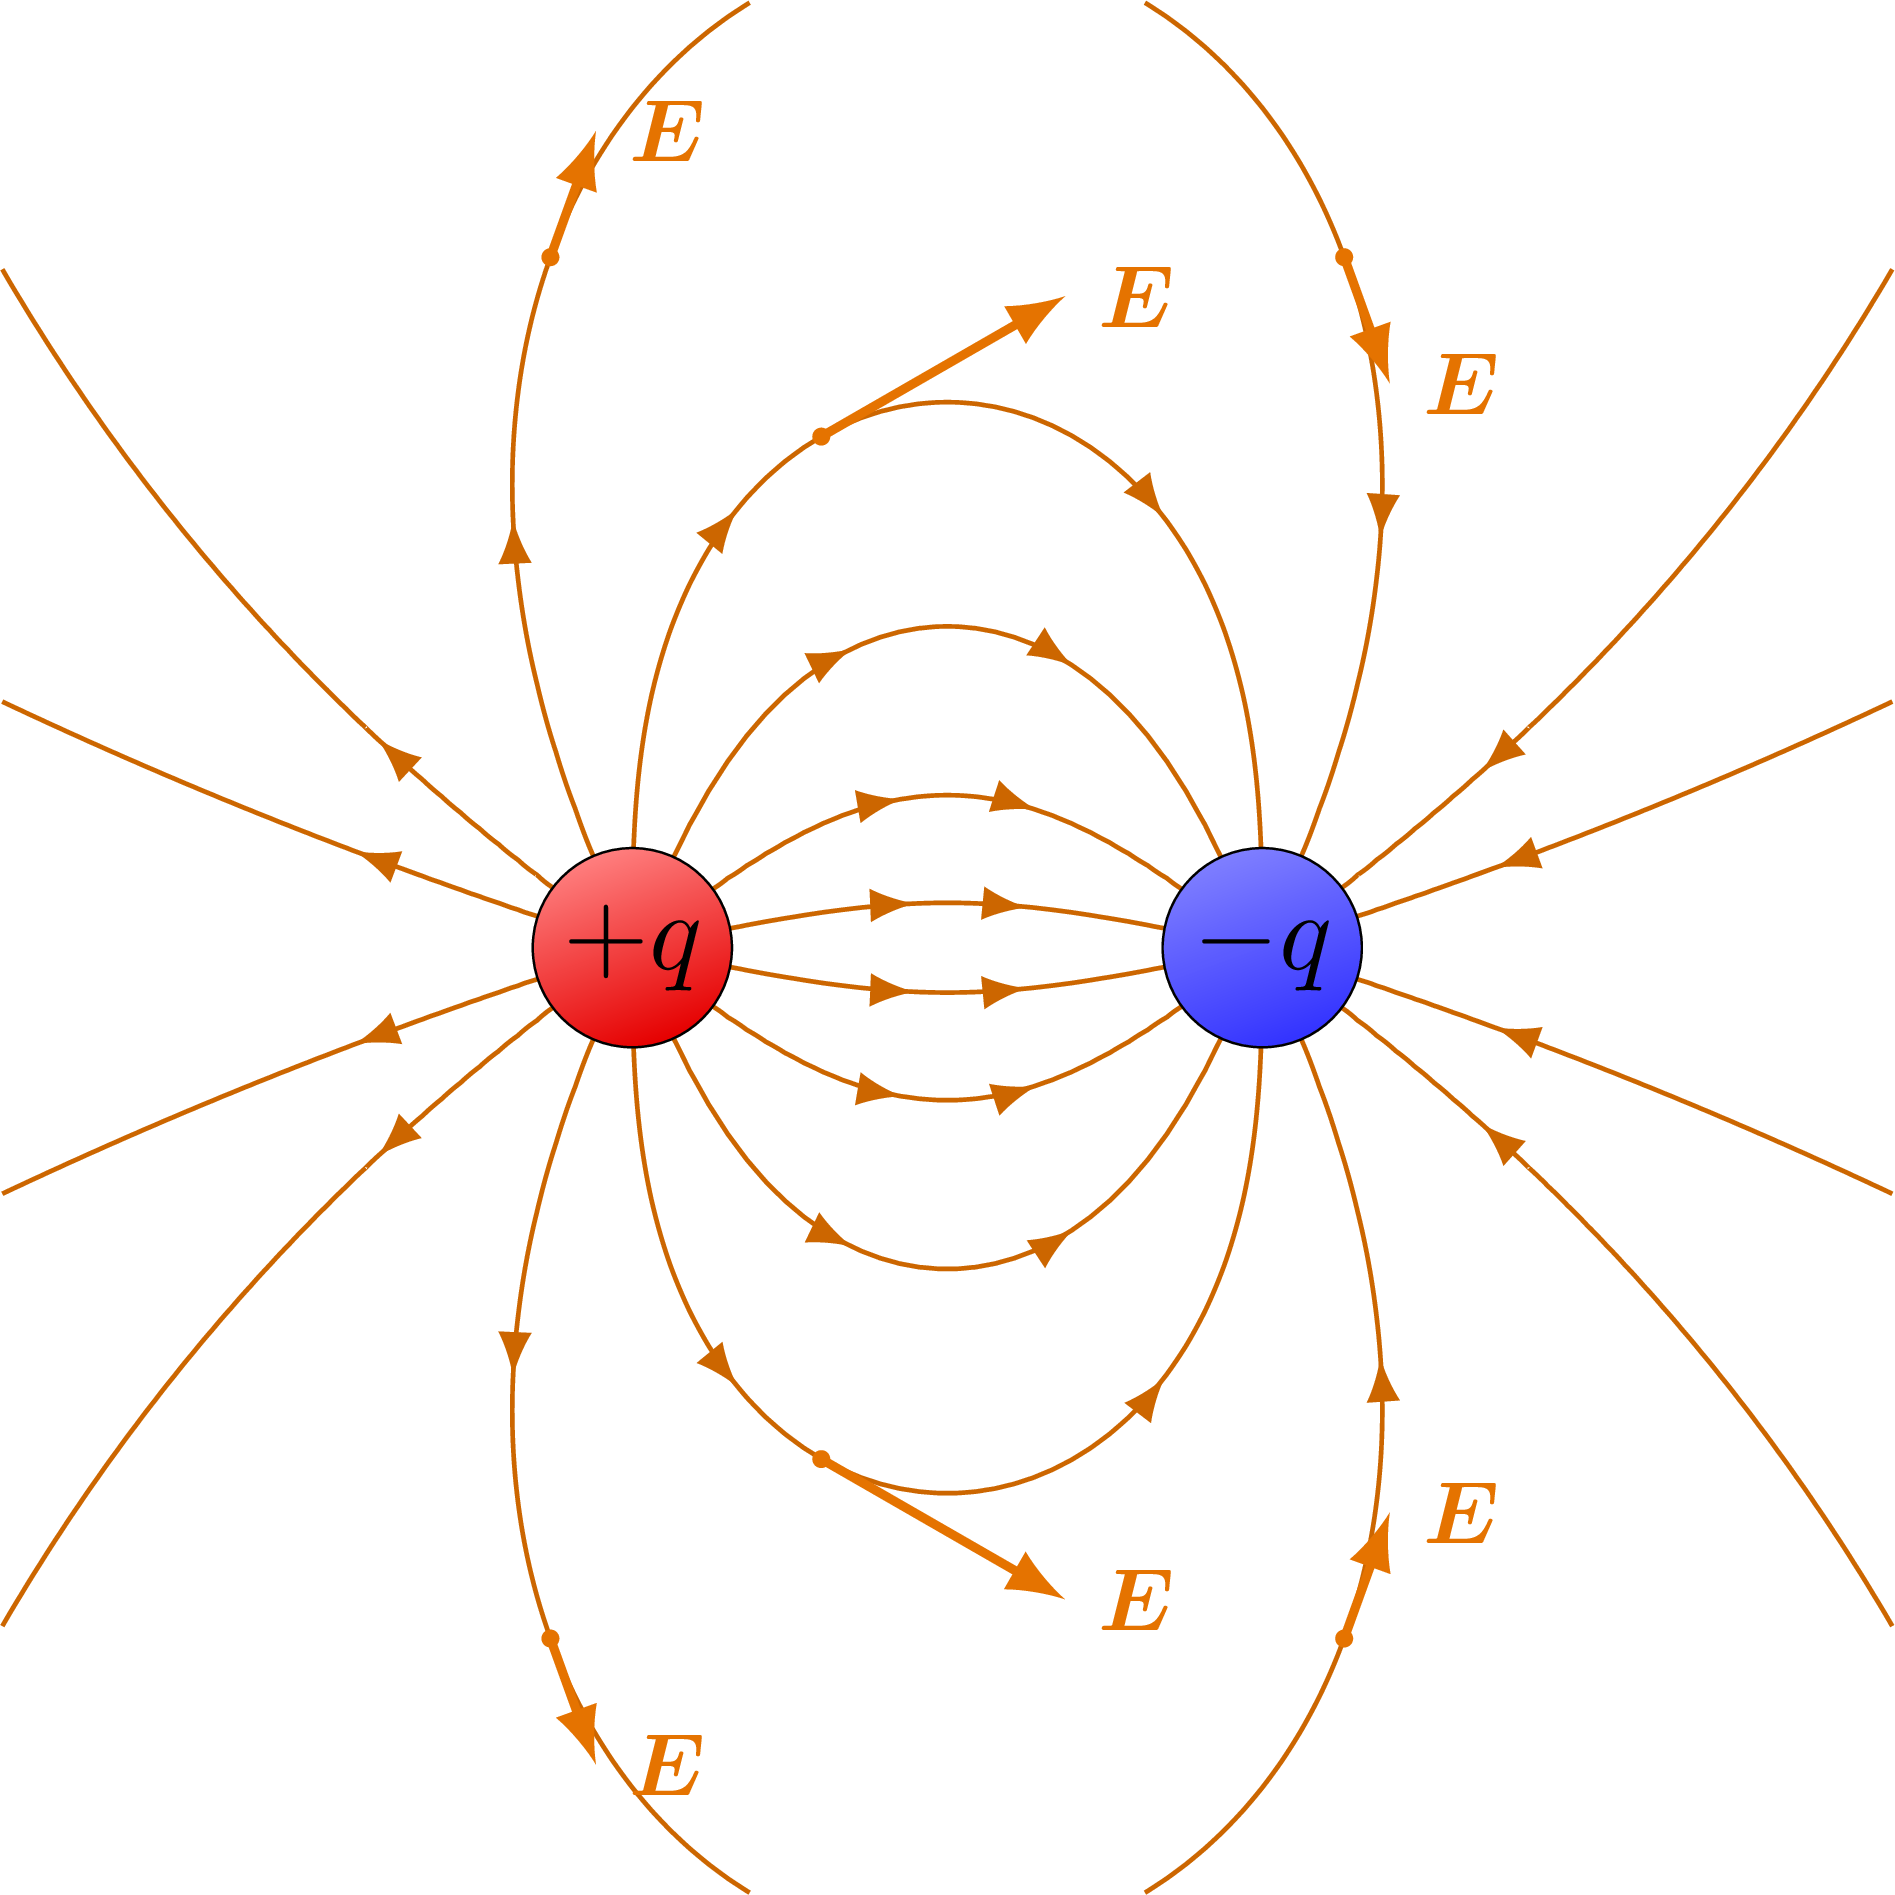
\includegraphics[width=.4\linewidth]{figures/electric_field.png}
	\caption{Electric field lines between a positive and negative point charge}
\end{figure}

The magnitude of the electric field at a given point in space with a singular point charge is equal to
\[
	\qty|\vec{E}| = \frac{k_{e} \qty|q|}{r^2} = \qty[\frac{N}{C}]
.\]

Note that for a point charge in a given electric field, the force on it can be written as
\[
	\vec{F}_{E} = q \vec{E}
.\]


Electric fields obey the superposition principle, meaning simply that the electric field at a point in space is equivalent to the vector sum of all the individual electric fields present at that point. Stated symbolically
\[
	\vec{E}_\text{total} = \sum_i \vec{E}_i
.\]


\end{document}
